%%%%%%%%%%%%%%%%%%%%%%%%%%%%%%%%%%%%%%%%%%%%%%%%%%%%%%%%%%%%%%%%%%%%%%
% Full Paper LaTeX2e Template for ``Genome Informatics 2003''        %
% Universal Academy Press, Inc.                                      %
%%%%%%%%%%%%%%%%%%%%%%%%%%%%%%%%%%%%%%%%%%%%%%%%%%%%%%%%%%%%%%%%%%%%%%

%%%%%%%%%%%%%%%%%%%  Read General Remarks  %%%%%%%%%%%%%%%%%%%%%%%%%%%
% 1. 11pt fonts should be used.                                      %
% 2. When special style files are used (e.g. epsf.sty),              %
%    please send the style files together.                           %
% 3. Even if color images are used, only black/white images          %
%    will be used for publication.                                   %
% 4. If you want to include figures in your article, please          %
%    use graphicx.sty or graphics.sty. You can take these macros     %
%    from our site in the same directory.(graphics.tar.gz)           %
%%%%%%%%%%%%%%%%%%%%%%%%%%%%%%%%%%%%%%%%%%%%%%%%%%%%%%%%%%%%%%%%%%%%%%

%%%%%  BEGIN Do not change  %%%%%%%%%%%%%%%%%%%%%%%%%%%%%%%%%%%%%%%%%%
\documentclass[twoside,11pt]{article}
\usepackage{graphicx}
\usepackage{makeidx}  % allows for indexgeneration
%
%\usepackage[dvips]{graphicx}    % needed for including graphics e.g. EPS, PS
\usepackage{epsfig}
\usepackage{url}
\usepackage{pseudocode}
\usepackage{comment}
\usepackage{array}
\usepackage{authblk}
\usepackage{color}
\usepackage{newalg}
\usepackage{subfigure}
\setlength{\topmargin}{-1cm}
\setlength{\oddsidemargin}{-0.5cm}
\setlength{\evensidemargin}{-0.5cm}
\setlength{\textwidth}{17cm}
\setlength{\textheight}{24cm}
\pagestyle{myheadings}
\author{}
\date{}
\setcounter{page}{1}
%%%%%  END Do not change %%%%%%%%%%%%%%%%%%%%%%%%%%%%%%%%%%%%%%%%%%%%%

%%%%%%%%%%%%%%%%%%%     \title    %%%%%%%%%%%%%%%%%%%%%%%%%%%%%%%%%%%%
\title{\bf
Bridging the gap: improving local multiple alignment with gapped extension.
}
%%%%%%%%%%%%%%%%%%%%%%%%%%%%%%%%%%%%%%%%%%%%%%%%%%%%%%%%%%%%%%%%%%%%%%

%%%%%%%%%%%%%%%%%%%   \markboth    %%%%%%%%%%%%%%%%%%%%%%%%%%%%%%%%%%%
\markboth{Treangen {\em et al.}}
         {Improving local multiple alignment with gapped extension}
% First  parameter: Single author         -> LastName1
%                   Two authors           -> LastName 1 and LastName2
%                   More than two authors -> LastName1 {\em et al.}
% Second parameter: Provide a short running head with length not
%                   greater than 45 letters.
%%%%%%%%%%%%%%%%%%%%%%%%%%%%%%%%%%%%%%%%%%%%%%%%%%%%%%%%%%%%%%%%%%%%%%


%%%%%  BEGIN Do not change  %%%%%
\begin{document}
\maketitle
\thispagestyle{myheadings}
\vspace{-1.8cm}
%%%%%  END Do not change %%%%%%%%

%%%%%%%%%% Author(s) and Email Address(es) %%%%%%%%%%%%%%%
% Remark: When paper is single authored, the affiliation %
%         need not be footmarked.                        %
%%%%%%%%%%%%%%%%%%%%%%%%%%%%%%%%%%%%%%%%%%%%%%%%%%%%%%%%%%
\begin{center}
%\begin{tabular}[t]{c}                      % One person in one line
\begin{tabular}[t]{c@{\extracolsep{2em}}c}  % two persons in one line
%\begin{tabular}[t]{c@{\extracolsep{2em}}c@{\extracolsep{2em}}c}
                                            % three persons in one line
  \bf    Todd  Treangen\footnotemark[1]
 &\bf    Aaron E. Darling\footnotemark[2]

\\
  \small\tt treangen@lsi.upc.edu
 &\small\tt a.darling@imb.uq.edu.au
%&\small\tt lastname3@disorder.chem.wsu.edu
\end{tabular}
\smallskip

%%%%%%%%%%%%% More Authors, if any %%%%%%%%%%%%%%%%%%%%%%%%%%%%
%\begin{tabular}[t]{c}                        % 1 person/line
%\begin{tabular}[t]{c@{\extracolsep{2em}}c}  % 2 persons/line
\begin{tabular}[t]{c@{\extracolsep{2em}}c@{\extracolsep{2em}}c}
                                             % 3 persons/line
  \bf    Guillaume Achaz\footnotemark[3]
&\bf    Mark A. Ragan\footnotemark[2]
&\bf    Xavier Messeguer\footnotemark[1]
%&\bf    FirstName5 MiddleName5 LastName5\footnotemark[3]
%&\bf    FirstName6             LastName6\footnotemark[3]

\\
\small\tt achaz@closun.snv.jussieu.fr
&\small\tt m.ragan@imb.uq.edu.au
&\small\tt peypoch@lsi.upc.edu
\end{tabular}
\smallskip
%%%%%%%%%%%%%%%%%%%%%%%%%%%%%%%%%%%%%%%%%%%%%%%%%%%%%%%%%%%%%%%



%%%%%%%%%%%%%%%%%%% Affiliation(s) %%%%%%%%%%%%%%%%%%%%%%%%%%%%
\begin{small}
\begin{tabular}{rl}
\footnotemark[1] & \parbox[t]{13cm}{
%%%%%%%%%% Affiliation for footnotemark[1] %%%%%%%%%%%%%%%%%%%%
Dept. of Computer Science, Technical Univ. of Catalonia, Barcelona, Spain
%%%%%%%%%%%%%%%%%%%%%%%%%%%%%%%%%%%%%%%%%%%%%%%%%%%%%%%%%%%%%%%
}\\
\footnotemark[2] & \parbox[t]{13cm}{
%%%%%%%%%% Affiliation for footnotemark[2] %%%%%%%%%%%%%%%%%%%%
Institute for Molecular Bioscience,
Univ. of Queensland, Brisbane, Australia
%%%%%%%%%%%%%%%%%%%%%%%%%%%%%%%%%%%%%%%%%%%%%%%%%%%%%%%%%%%%%%%
}\\
\footnotemark[3] & \parbox[t]{13cm}{
%%%%%%%%%% Affiliation for footnotemark[3] %%%%%%%%%%%%%%%%%%%%
Atelier de Bioinformatique, Univ. Pierre et Marie Curie-Paris 6, Paris, France
%%%%%%%%%%%%%%%%%%%%%%%%%%%%%%%%%%%%%%%%%%%%%%%%%%%%%%%%%%%%%%%
}\\
\end{tabular}
\end{small}
\bigskip
\end{center}

%%%%%%%%%%%%%%%%%%     Abstract   %%%%%%%%%%%%%%%%%%%%%%%%%%%%%
\begin{abstract}
The identification of homologous DNA via sequence alignment is a basic building block in comparative genomics.  We present a method for accurately and sensitively identifying homologous DNA sequence in multiple genomes. Our method is based around an efficient heuristic for local multiple alignment, featuring a novel method for gapped extensions. In practice, we are able to sensitively identify conserved, potentially repetitive, regions in one or more DNA sequences.  The GPL implementation of our algorithm in C++ is
called \texttt{procrastAligner} and is freely available from: \url{http://alggen.lsi.upc.es/recerca/align/procrastination/}

\end{abstract}
%%%%%%%%%%%%%%%%%%%%%%%%%%%%%%%%%%%%%%%%%%%%%%%%%%%%%%%%%%%%%%%

\noindent {\bf Keywords:}
%%%%%%%%%%%%%%%%%%%%%%%%  Keywords %%%%%%%%%%%%%%%%%%%%%%%%%%%%
sequence alignment
%%%%%%%%%%%%%%%%%%%%%%%%%%%%%%%%%%%%%%%%%%%%%%%%%%%%%%%%%%%%%%%



%%% BEGIN CONTENTS %%%
\section{Introduction}

The importance of accurate homology identification to comparative genomics can not be overestimated~\cite{Kumar07}. To date, pairwise local sequence alignment methods~\cite{ref-blast, ref-ssearch} have been the prevailing technique to identify homologous nucleotides.  When more than two copies of a homologous sequence element are present in the data, pairwise homology detection methods generate a listing of all possible pairs of homologous elements.  Apart from the obvious inefficiency of considering all pairwise homology relationships, a collection of pairwise alignments is not ideal because they are rarely amenable to comparative genomic and phylogenetic analysis without further processing into a multiple alignment.

Local pairwise alignments can be merged to create a multiple alignment by a variety of methods~\cite{ref-tba,ref-aba,ref-dialign,ref-related1}. Such methods commonly assume that pairwise homology relationships are transitive, such that if nucleotide $a$ is homologous to nucleotide $b$, and $b$ is to $c$, then $a$ must also be homologous to $c$.  Thus, in order to merge pairwise alignments, such methods must tackle the challenging problem of resolving inconsistent transitive homology relationships.  Pairwise alignment has been demonstrated to be less accurate than multiple alignment, especially when dealing with a large number of divergent sequences~\cite{ref-mlagan,ref-aubergene}.  As the number of homologous sequences grows, we might expect that the number of inconsistent relationships in a collection of pairwise alignments would grow quadratically, whereas a direct multiple alignment method would provide an increasingly accurate alignment.  Highly repetitive regions in the input sequences can cause particularly nasty efficiency problems for pairwise methods, as they create $O(r^{2})$ pairwise alignments in the presence of a repeat with $r$ copies.  Mammalian Alu repeats and IS elements in microbes are just two common examples of the overwhelming abundance of repetitive sequence in naturally occurring genomes.

Local multiple alignment has the inherent potential to avoid pitfalls associated with pairwise alignment. Although optimal multiple alignment under the SP objective function remains intractable~\cite{ref-wangjiang}, progressive alignment heuristics offer excellent speed and accuracy~\cite{ref-clustalw, ref-tcoffee} especially when combined with tree-independent iterative refinement~\cite{ref-muscle}. Rather than merging pairwise alignments, why not exploit years of research into multiple alignment heuristics by directly constructing a multiple alignment?   In the context of \textit{local} multiple alignment, the fundamental problem with such an approach is that current methods for progressive alignment with iterative refinement compute \textit{global} alignments, i.e. they implicitly assume that input sequences are homologous over their entire length.

We present a novel heuristic for directly computing local multiple alignments that exploits the MUSCLE multiple alignment algorithm to compute gapped extensions of seed matches.  Our method assumes that a fixed number of nucleotides flanking a seed match is likely to be homologous and computes a global multiple alignment on the flanking region.  In some cases our assumption of flanking homology proves erroneous and results in an alignment of unrelated sequences.  We apply random walk statistics to detect any such non-homologous regions embedded in the global multiple alignment.  Non-homologous regions are then removed from the alignment and the local-multiple alignment is trimmed to reflect the updated boundaries of homology.  The remainder of this manuscript presents details of our computational approach, an evaluation of the accuracy of our method on synthetic datasets, and an application to Alu genome data.



\label{sec:overview}
\section{Definitions and Notation}

Given a sequence $\mathcal{S}=s_1, s_2,\dots, s_N$ of length $N$
defined over an alphabet $\{A,C,G,T\}$, our goal is to identify all homologous nucleotides in $\mathcal{S}$.
Since we assume that homology is a transitive property, all 
local multiple alignments on subsequences of $\mathcal{S}$. We denote
an ungapped alignment, or match, among subsequences in $\mathcal{S}$
as an object $M$, and a set of such matches as $\mathbf{M}$.
We refer the number of regions in $\mathcal{S}$
matched by a given match $M_i \in \mathbf{M}$ as the
\textit{multiplicity} of $M_i$, denoted as $|M_i|$. There is a limitation on the matches in
$\mathbf{M}$, no two matches $M_i$ and $M_j$ may have the same
left-end coordinate.  This constraint has been referred to by others as \textit{consistency} and
\textit{transitivity}~\cite{ref-transitivity} of matches.  In the
present work we only require consistency and transitivity of matches
longer than the seed length, e.g. seed matches may overlap. We denote a gapped alignment, or local alignment, among subsequences in $\mathcal{S}$ as $A$, and a set of gapped alignments as $\mathbf{A}$.  In practice, each $A_i$ in $\mathbf{A}$ is constructed via
at least one $M_i$ in $\mathbf{M}$. When $|M_i|>2$,$|A_i|>2$ we refer to $M_i$,$A_i$ as
a multi-match and a multiple local alignment, respectively.  

The sum of pairs objective function used is defined as follows:\\
%\begin{equation}

$$
\begin{array}{l}
f(i,0) = 0,\\
f(0,j) = 0,\\
\end{array}
f(i,j)= \max\left\{\begin{array}{l}
f(i,j) = f(i-1,j-1)+\mu_{ij},\\
f(i,j-1) - \gamma\\
f(i-1,j)-\gamma\\
0 \\
\end{array}\right.
$$
\begin{center}
$\mu_{ij}$ is the mismatch score between positions $i,j$ in $\mathcal{S}$.  $\gamma$ is the fixed gap penalty.
\end{center}
%\end{equation}

\section{A heuristic for local multiple alignment}
Because the cost of alignment in multiple sequences grows exponentially with respect to the number of sequences, we must find clever ways to perform and limit the amount of gapped alignment via dynamic programming that is performed. Gapped alignments arise when trying to extend seeds to fully capture surrounding sequence homology. Our aim is to bridge this gap in efficiency by presenting a novel heuristic for gapped extension for sensitive local multiple alignment.

Our heuristic for local multiple alignment, as depicted in Figure~\ref{fig-main},
can be divided into five independent steps:
(1) detection of multi-matches using palindromic spaced seeds
(2) prioritized chaining of all multi-matches
(3) gapped extension of all chains
(4) estimation of homologous sequence boundaries using random walk statistics
(5) unalignment of all non-homologous sequence in local multiple alignment

\begin{figure}[t]
\centering 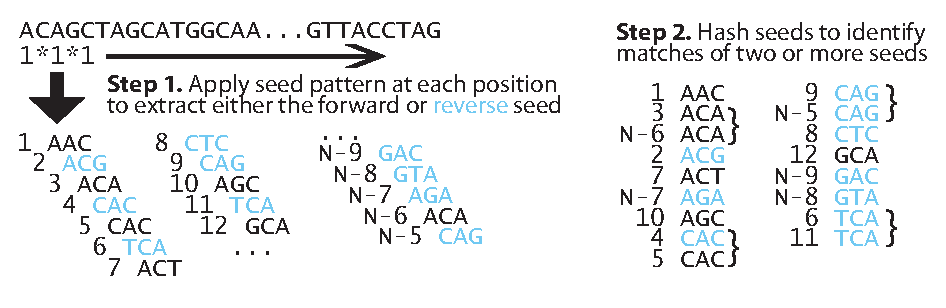
\epsfig{file=./figures/string_matching.eps,width=5.2in}
\caption{Application of the palindromic seed pattern
\texttt{1*1*1} to identify degenerate matching subsequences in a
nucleotide sequence of length $N$. The lexicographically-lesser of
the forward and reverse complement subsequence induced by the seed
pattern is used at each sequence position.}

\label{fig-seeds}\vspace{-0.2cm}
\end{figure}

\begin{figure}
\begin{center}
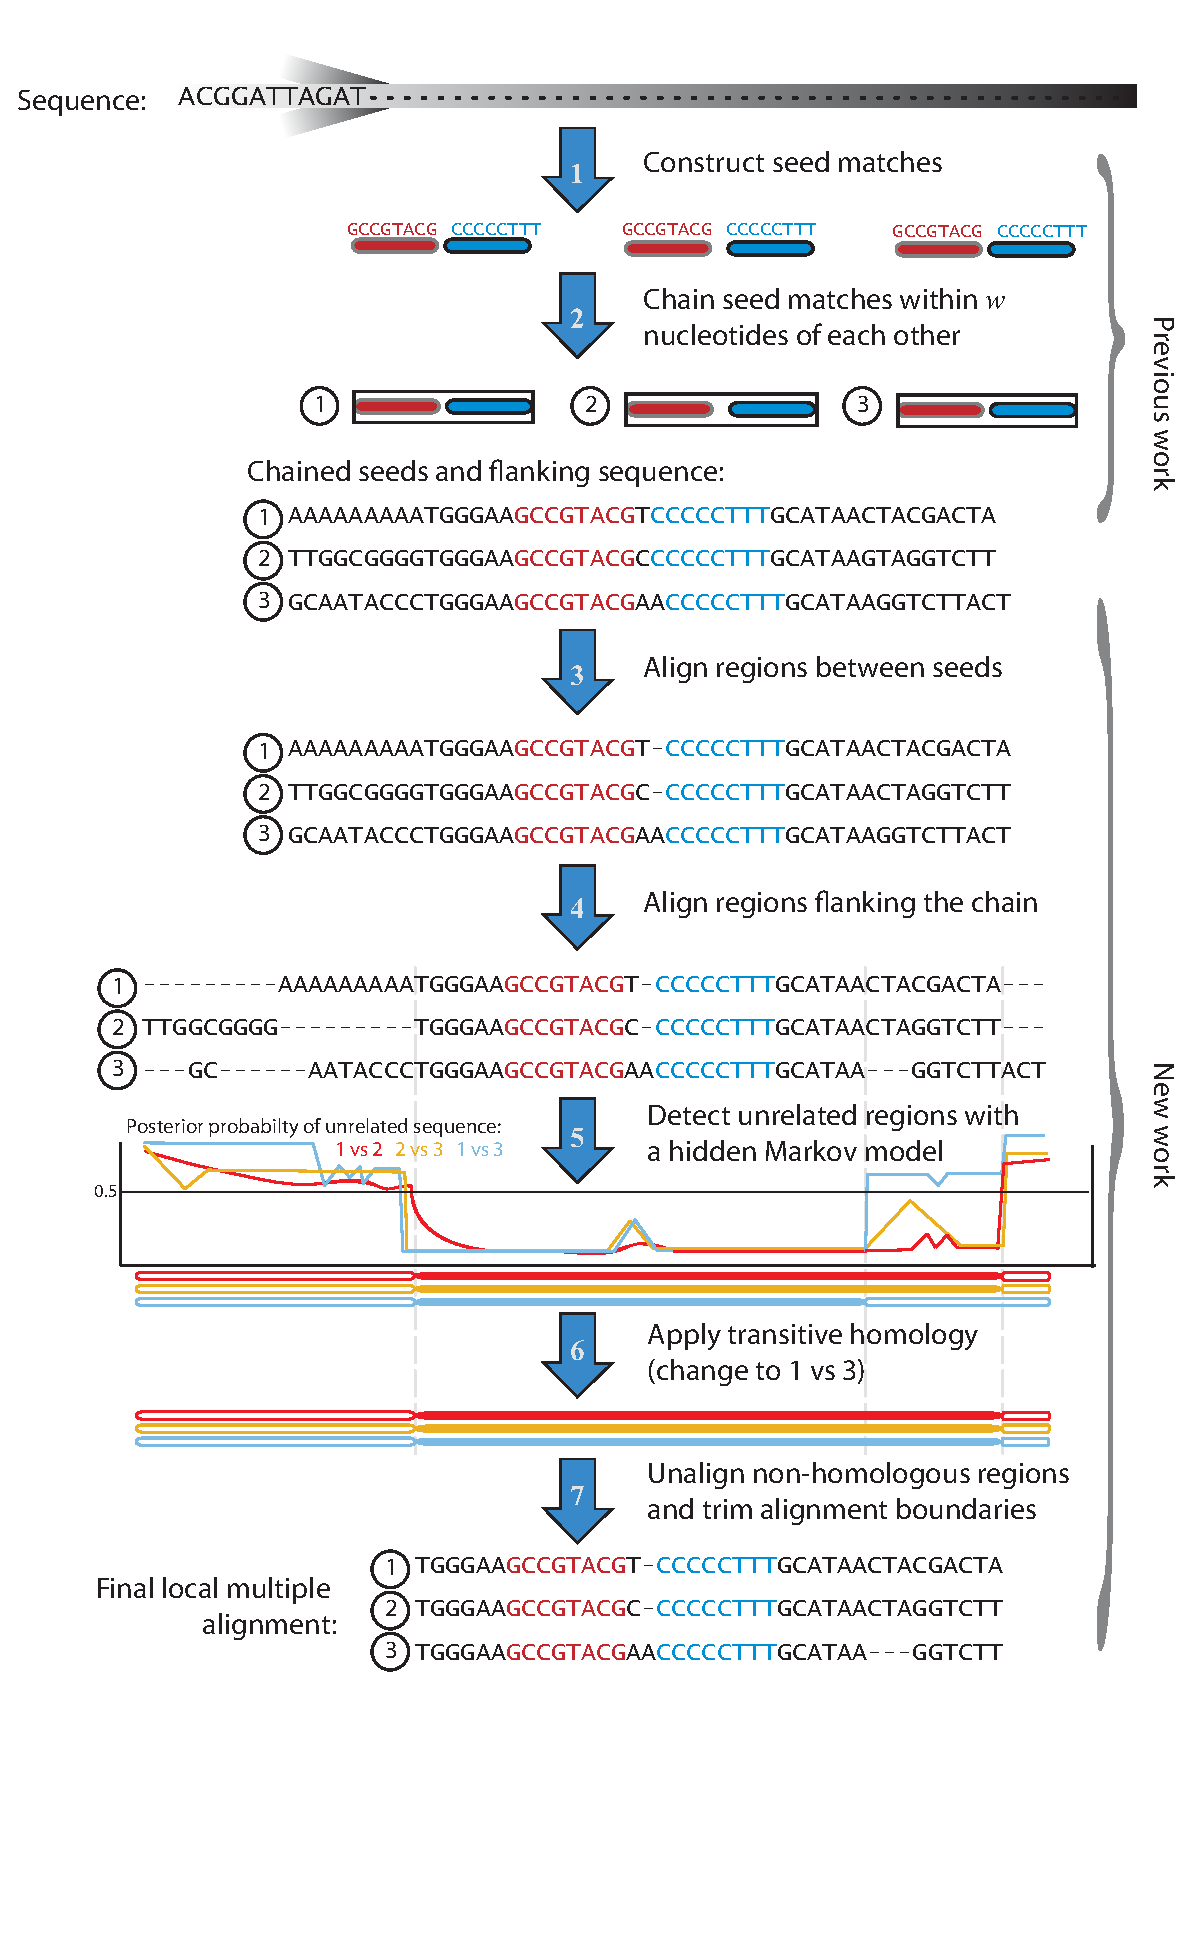
\epsfig{file=./figures/extension.eps,width=5.0in}
%\subfigure[Visual representation of our algorithm]{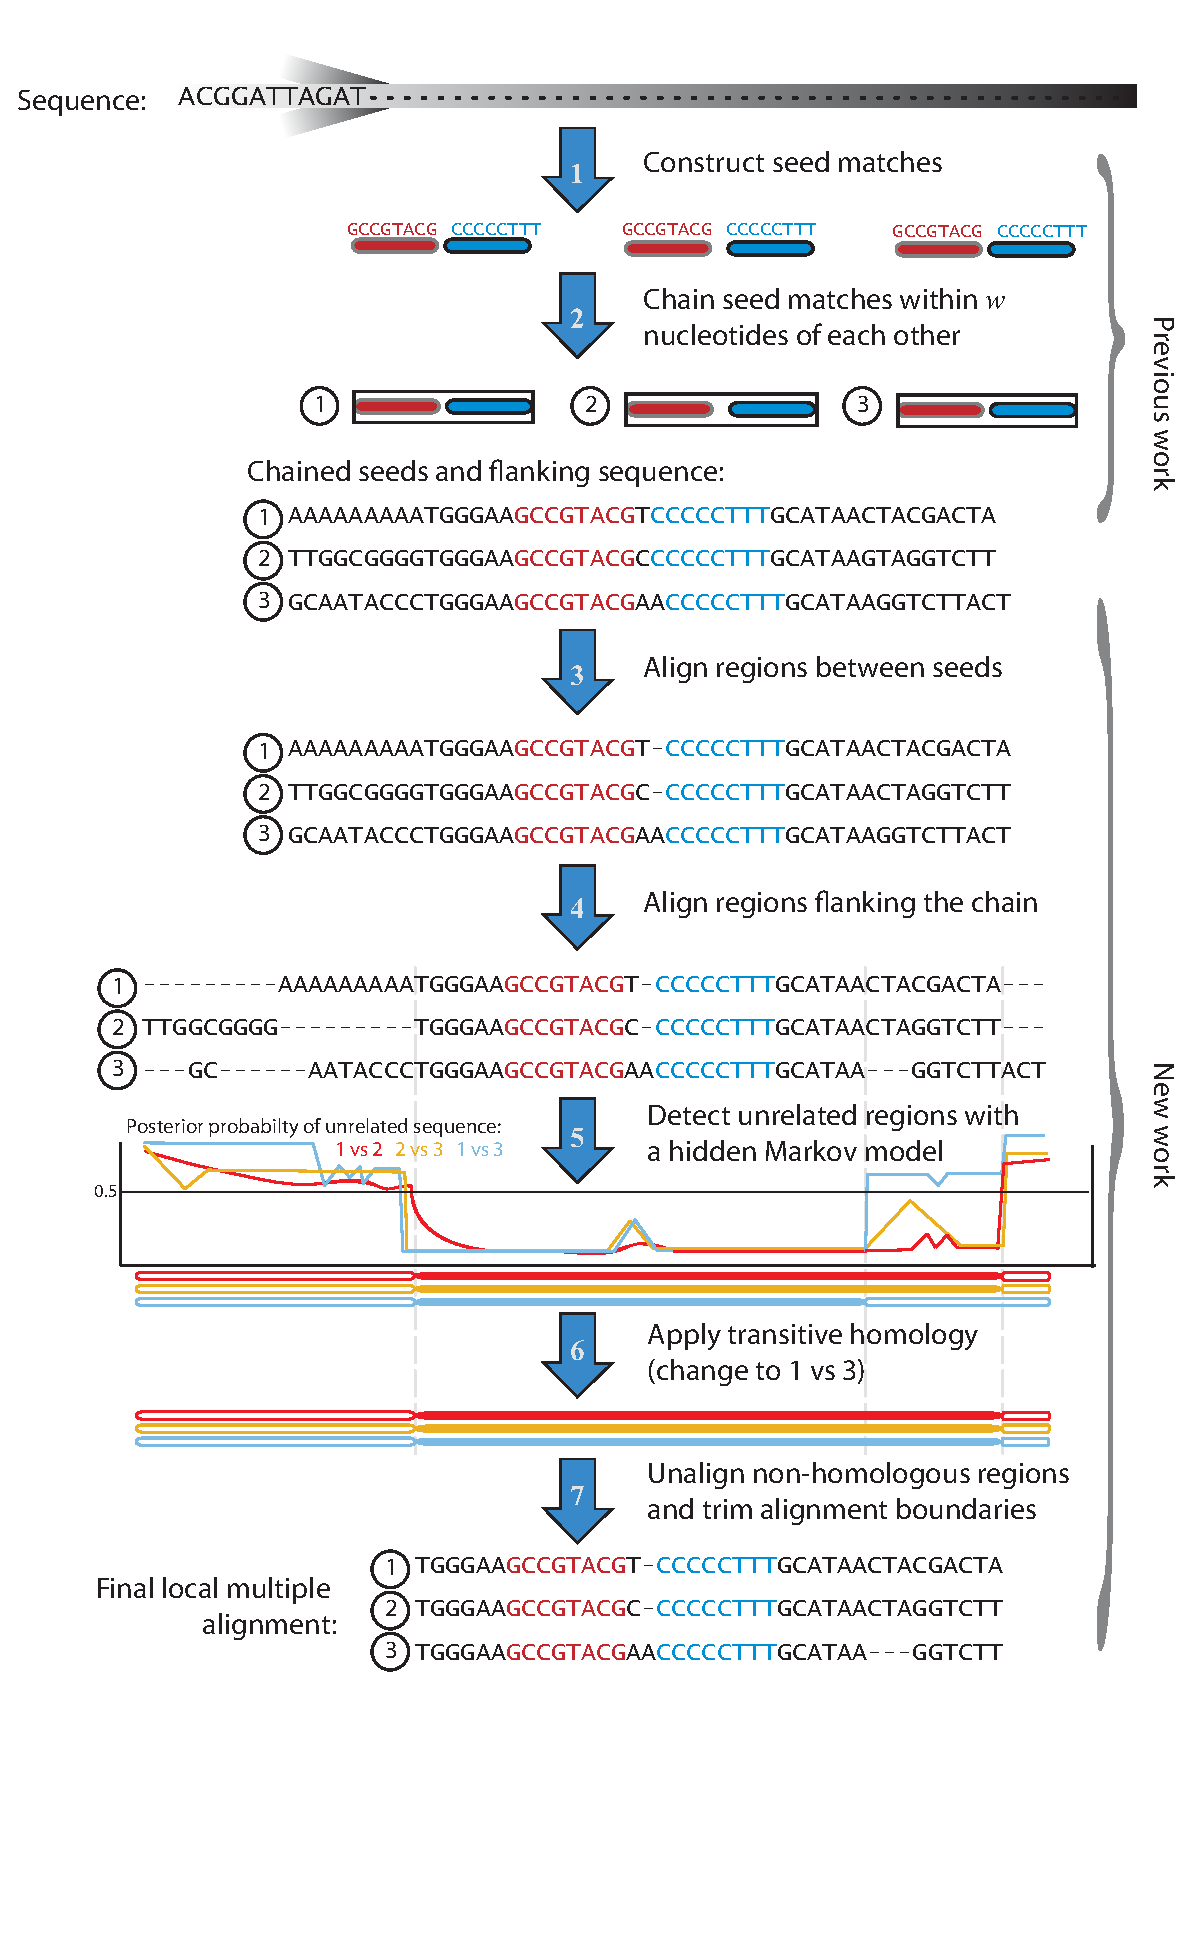
\epsfig{file=./figures/extension.eps,width=3.0in}}
%\subfigure[Flowchart of the algorithmic process ]{ 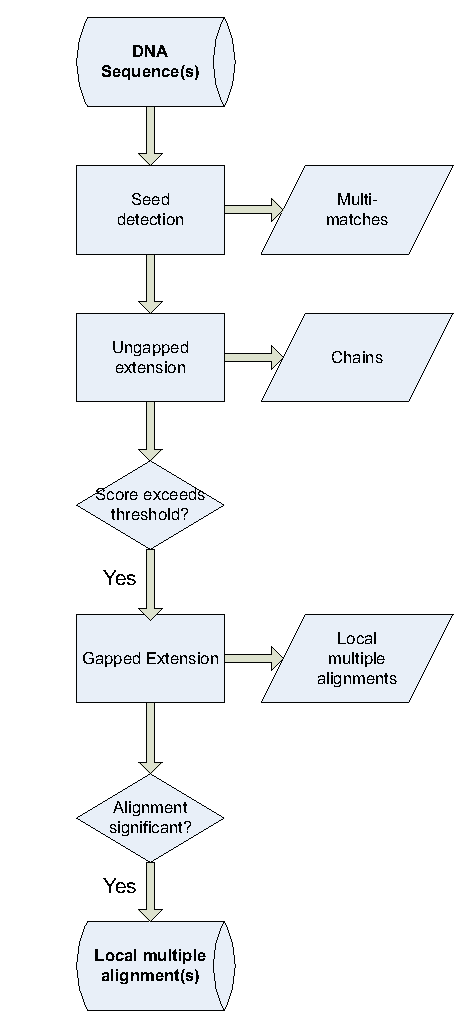
\epsfig{file=./figures/flowchart.eps,width=1.7in}}
\end{center}
\caption{Overview of the method, starting with an input sequence and ending with a set of local multiple alignments. First we (1) detect multi-matches in input sequence(s) using palindromic spaced seeds, then we perform (2) prioritized chaining of all multi-matches.  The resulting chain contains two matches and three match components labeled 1, 2, and 3.  We then perform gapped alignment of the region between chained matches (3).   In step (4), we perform a gapped extension by computing a global multiple alignment on the regions to the left and right of each chain component.  The resulting alignment may contain non-homologous sequence, so in step (5) we apply random-walk statistics to detect poorly aligned regions indicative of unrelated sequence.  In step (5), heavily diverged homologous sequences may be incorrectly classified as nonhomologous.  Step (6) computes transitive homology relationships to ensure a consistent alignment and aid detection of divergent homologous sequences.  Finally, in step (7) we unalign regions found to be non-homologous.  If we find after step (7) that the alignment boundaries have been extended, we acquire additional flanking sequence and return to step (4) for another round of extension.}
\label{fig-main}
\end{figure}


%\colorbox[named]{Gray}{adfa}

\subsection{Detecting seed multi-matches}

As a starting point for homology detection, we locate all spaced seeds of a given weight $z$ in the input sequence(s). The palindromic spaced seed pattern is analyzed at each position in the input sequence to identify all multi-matches (see Figure~\ref{fig-seeds}).  Previously we have demonstrated that palindromic spaced seeds offer good efficiency and sensitivity on a variety of input sequences~\cite{ref-procrast}.

\subsection{Creating chains of multi-matches}

Once we have generated a list of multi-matches, we rely on our previously described method for efficiently filtration method for chaining ~\cite{ref-procrast}. A brief review of the method follows(for additional details refer to the manuscript).

In order to chain over each region of sequence $\mathcal{O}(1)$ times,
our method chains matches in order of decreasing multiplicity--we
extend the highest multiplicity matches first. When a match can no
longer be chained without including a gap larger than $w$
characters, our method identifies the neighboring \textit{subset}
matches within $w$ characters. We then \textit{link} each
neighboring subset match to the chained match. We refer to the
chained match as a \textit{superset} match. Rather than immediately
extend the subset match(es), we \textit{procrastinate} and extend
the subset match later when it has the highest multiplicity of any
match waiting to be extended. When chaining a match with a linked
superse, we
immediately include the entire region covered by the linked superset
match--obviating the need to re-examine sequence already covered by
a previous match extension.

Once we have finished the chaining process, we would like to score and evaluate the chained multi-matches to make a decision whether its worth spending computational resources on gapped extension. This idea has been used in other local multiple alignment heuristics~\cite{...} in order to minimize the number of gapped extensions that do not improve the boundaries of the chain.

\subsection{Gapped extension of high scoring chains}

Now that we have decided to performed a gapped extension in the current direction, we use MUSCLE to align the left/right region immediately surrounding the chains. The size of the extension window we send to MUSCLE is the lesser of 4*w or 200 nucleotides. The reasoning by setting our minimum extension window to 200nt is closely related to how we determine homology borders. Since we will assume that the extension window we have decided to align with MUSCLE is homologous over its entire length, we use random walk statistics to correct our assumption.

\subsection{Identifying non-homologous regions}

The MUSCLE alignment software dutifully reports the highest scoring global multiple alignment of input sequences, regardless of whether they are homologous.  When MUSCLE aligns partially or wholly unrelated sequences, the alignment scores in the unrelated region take on negative values, as dictated by the HOXD scoring matrix and associated substitution and gap open penalties.  Random-walk statistics require a cumulative score function that trends toward negative values, but seeded alignments are expected to have large positive scores on average.  Thus, we simply invert the scoring scheme so it assigns negative values to matches and positive values for substitutions and gaps to arrive at a score with a negative expected value for seeded alignments.

When applying random walk statistics, we consider each pair of aligned sequences separately.  Given the scoring scheme, the cumulative sum of scores can be calculated for each pair of aligned nucleotides:

\begin{equation}
\label{eqn:scoresum}
S_n^\theta(a) = \sum_{i=1}^{n} Score_\theta(a_i) = S_{n-1}^\theta(a) + Score_\theta(n), S_0^\theta = 0
\end{equation}

Since the expected value $E(\theta) < 0$, partial score sums generate transient random walks.  Random stopping times can be defined recursively as:
\begin{equation}
\label{eqn:stoppingtimes}
\tau_0 = 0, \tau_1 = \min_i(S_i < S_0),\dots,\tau_{k+1} = \min_i(S_i < S_{\tau_k})
\end{equation}
where $S_n$ is defined as in Eqn.~\ref{eqn:scoresum}.  The random stopping times defined by $\tau$ form a strictly decreasing set of ladder points.  The horizontal distances (in alignment columns) between consecutive ladder points $\tau_{k+1}-\tau_{k}$ are referred to as ladder epochs.

We refer to the maximum score achieved during the $k^{th}$ ladder epoch as the Local Record Height for that epoch, as defined by:
\begin{equation}
\mathrm{LRH}_k = \max_{\tau_{k-1}\leq t \leq \tau_k}(S_t - S_{t_{k-1}})
\end{equation}
FIXME: one of the previous should be arg\{max/min\} instead of \{max/min\}.  Note that $\mathrm{LRH}_k \geq 0$.  The number of ladder epochs in an alignment with $N$ columns is denoted as $\wedge(N)$.  The distribution of the maximum value in a sequence of local record heights generated on an alignment can be approximated by an Extreme Value Distribution (EVD) parameterized as:
\begin{equation}
\label{eqn:evd}
Pr(\max_{j \leq \wedge(N)}(\mathrm{LRH}_j > x)) = \exp(-NKe^{-\mu x})
\end{equation}
Here $\mu$ is the positive solution of an equation involving the moment generating function that accounts for sequence composition and indel frequency:
\begin{equation}
mgf_\theta(\mu) = \sum_j \pi_j e^{\mu \theta\{j\}}
\end{equation}
For the HOXD substitution matrix and associated affine gap penalties this equation takes the form $mgf_\theta(\mu) = \pi_{A\leftrightarrow A}e^{91\mu} + \pi_{C\leftrightarrow C}e^{100\mu} + \pi_{G\leftrightarrow G}e^{100\mu} + \pi_{T\leftrightarrow T}e^{91\mu} + \pi_{A\leftrightarrow C}e^{-114\mu} + \pi_{A\leftrightarrow G}e^{-31\mu} + \pi_{A\leftrightarrow C}e^{-123\mu} + \pi_{C\leftrightarrow G}e^{-125\mu} + \pi_{C\leftrightarrow T}e^{-31\mu} +  \pi_{G\leftrightarrow T}e^{-114\mu} + \pi_{gapopen}e^{-400\mu} + \pi_{gapext}e^{-35\mu}$; where $\pi_j$ is the observed frequency of a column of type $j$ in the alignment.  FIXME: is this right and does it work correctly for gaps?

We estimate the values of $K$ and $\wedge(N)$ from Equation~\ref{eqn:evd} by recording the maximum LRH values observed in each each of 10,000 simulations and then fitting the functional form of Equation~\ref{eqn:evd} to the resulting distribution of extreme values.  FIXME: need to incorporate Guillaume's GC content approximation here?

Solving for $\mu$ and subsequent application of Equation~\ref{eqn:evd} enables us to deduce an approximate scoring threshold beyond which the ladder epoch in question contains non-homologous sequence with probability greater than a chosen value.

Although we can be nearly certain that ladder epochs with a LRH exceeding our significance threshold contain an alignment of non-homologous sequence, the exact columns where the transitions between homology and non-homology take place remain ambiguous.  To determine tight boundaries on the non-homologous region, we compute ladder points for the significant region in the forward and reverse direction and call the entire region between ladder points non-homologous.

The result of applying the random-walk statistics is a prediction of non-homologous segments among each pair of aligned sequences.  The remaining regions are predicted as homologous.  We apply transitivity to these homology predictions, resulting in a final set of consistent homology predictions.  See Figure~\ref{fig:example}, steps 5 and 6 for an example. Regions found to be non-homologous are unaligned from each other.


\textbf{FIXME}: we can exceed the threshold and still improve boundaries.  If have reached the end of the extension window without going beyond our homology threshold, we then improve our original seed boundaries and then trigger another round of chaining(and consequently another round of extension) in the same direction on the currently active, extend match. Else, if we surpass the homology threshold we first determine if our chain boundaries have been improved, and then signal that we are done chaining/extending the current match in the current direction. If we have already processed the current chain in both directions, we stop entirely and proceed to the next multi-match in the priority queue.

%\subsubsection{Processing Novel homologous sequence}
%Its worth mentioning that novel homologous sequence can be found during gapped extension.
%FIXME: should briefly describe what we do with this!

\subsection{Assigning significance to local multiple alignments}
FIXME: insert statistics here!

\section{Results}
We have created a program called \texttt{procrastAligner} for Linux, Windows, and Mac OS X that implements the described algorithm. Our
open-source implementation is available as C++ source code licensed under the GPL. As input, \texttt{procrastAligner} accepts FastA and multi-FastA DNA sequences. As output, the program returns a XMFA formatted file of all significant local multiple alignments. Figure~\ref{fig-align} shows an example local multiple alignment generated with \texttt{procrastAligner}.


\begin{figure}[t]
\scriptsize
\begin{verbatim}
CAGCTACTTGGGAGGCAGAGGTGGGAGGATTGCTTGAACCTG--------GAGATTCAAGTGAGCTGAGATTGCACCACTGCATTCCAGCCTGGGC--AACAAAGCAAGACTCT-
CAGCTATTCAGGAGGCTGAGGCAGGAGAATTGCTTGAACCTGGGAG-GCGGAGGTTGCAGTGAGCCGAGATGACGCCACTGCACTCCAGCCTGGGC--GACAGAGCA--------
CAACTACTCAGGAGGCTGAGGCAGGAGAATCGCTTGAACCCAAGAGAGTGAAGGTTGCAGTGAGCTGAGATCATGCCACTTCACTCCAGCCTGAGTGAAACAGC-----------
CAGC------------------AGGAGAATAACTTCAACCTGGGAG-ACAGAGGTTGCAGTCAGCTGAGATCGCACCACTGCATTCCAGCCTGGGT--GACAGACCGAGACTCTG
CAGCTACTTGGGAGGCTGAGGCAGGAGAACTGCTTGAACTCGGGAG-GCAGAGATTGCAGTGAGCTGAGATCATGTCAATGCACTGCAGCTTGAGT--GACAGAGTG--------
CAGCTACTAGGGAGGCTAAGGCAGGAGAATCGCTTGAACCTGGGAG-GCAGAGGTTACAGAGAGCTGGGATTGTGCCACTGCACTCCGGCCTGGGC--AACAGAATG--------
CAGCTACTCAGGATGCTAAGGCA-CAGAATCACTTGAACCTGGGAG-GCAGAGGTTACAGTGAGCCAAAATCGCGCCACTGCACTCCAACCTGGGC--AACACAGCAA-------
CAGCTACTCAGGAGGCTGAGGCAGGAGAATTGCTTGAACCCGGGAG-GTGGAGGCTGCAGTGAGCCGAGATCATGCCACTGCACTCCAGCCT-GGT--GACAGAGCGAGA-----
CAGCTACTCGGGAGGCTGAGACAGGAGAATTGTTTGAACCCAGGAG-GCGGAGGCTGCAGTGAGCCGAGATTGTGTCACTGTACTCCAGCCTGGGCAAGACAGAG----------
CTGCTACTCAGGAAGCTGAGGCAGGAGAATCCCTTCAACCTGGGAA-ACAGAGGTTGCAGTGAGCCAAGATCGCACCATTGCACTCCAGTCTGGGC--AACAGAGAGA-------
*  *                     ** **   ** ***            *   *  * * * *    *  *   ** *  *  **            * *
\end{verbatim}
\vspace{-0.5cm}
\normalsize
\caption{Partial alignment of Alu-Sc subfamily found in \emph{H. sapiens} C1 esterase inhibitor gene. Each row represents an aligned ALU.}.
\label{fig-align}
\end{figure}

\subsection{Retrieval of randomly generated motifs}
%describe and present results(table)
Comparison with EulerAlign, HomologMiner, MultiZ, and RepeatScout??


We have previously demonstrated the sensitivity of our chaining method in finding Alu repeats in
the human genome~\cite{ref-procrast}. To highlight the benefits of our proposed heuristic for gapped extension, we have inserted mutated copies of randomly generated patterns into \emph{Mycoplasma genitalium}. \emph{M. genitalium} has been recognized as a complex and repeat rich genome, presenting a biologically relevant and challenging example to evaluate our method. Specifically, we used a 6 step process to generate and insert artificially generated DNA patterns into the genome is as follows. First, we randomly choose a pattern length, between 20nt and 200nt (\textbf{is this random from a uniform distribution of lengths?}). Then, we randomly choose a nucleotide for each column of the pattern (\textbf{what is the background frequency of A/C/G/T?}). After we have generated the pattern, we then randomly selected a multiplicity/copy number for the pattern (between 20 and 300 copies). We configured the process to make it less likely for larger patterns to have higher multiplicities, and vice versa \textbf{give the equation}. Then, we randomly mutated each copy of the pattern using substitutions and indels. The substitution and indel frequency were configured to 0.0x. Afterwards, we randomly placed each copy either on the forward or reverse strand. Finally, we randomly selected the minimum distance between any two copies (between 100-1000nt)\textbf{uniform distribution?}. Again, we made it more likely for smaller patterns to be located further apart, and larger patterns closer together\textbf{why?}. We then used \texttt{procrastAligner} to find all significant multiple local alignments in the modified genome of \emph{M. genitalium} and recorded whether it was able to fully recover all mutated copies of the  artificially generated pattern. Then we compared \texttt{procrastAligner}'s performance to that of two related programs, EulerAlign~\cite{ref-related1} and HomologMiner~\cite{ref-homologminer}, by evaluating each program's ability to accurately recover the inserted patterns via their multiple local alignment heuristic. Results of this experiment are reported in Table~\ref{tab-results}.

\textbf{note from AED:}\textit{Another possibility would be to generate, say, 10 patterns for each multiplicity between 20 and 300 (or 2 and 300), then plot the change in sensitivity/specificity as a function of multiplicity.  It would also be nice to see how Sn/Sp vary as a function of sequence divergence.  For example, we could try a range from 0 substitutions per site (no divergence) to 1 or 2 substitutions per site.  Since we're modeling all sites to be equally likely to accept a substitution, we would expect procrastAligner to totally break down before we get to 1 substitution per site.  A common refinement to these models assumes that some sites are more likely to mutate than others, and this is typically modeled using a gamma distribution (aka gamma-distributed rate heterogeneity).}

\begin{table}[t!]
\scriptsize
  \centering
\begin{tabular}{|lccccc|rccccc|}
\hline ID & Length & Copies & Indels & Subs & Inversions & Method & Sn \% & Sp \% & T (s) & Sw & $w$ \\
\hline
\hline Pattern1 &  49 nt &  42 & 1 & 1 & 0 & EulerAlign & 100 & 97.3 & 324 & 9 & - \\
%&&&&&                                           & MultiZ & 100 & 97.3 & 324 & 9 & - \\
\multicolumn{6}{|c|}{\tiny ATCCTAGTCTAGAATTATTTATTCAGTTAGTTTCTACGAAGATGAACAAT}& procrastAlign & 100 & 93.6 & 188 & 9 & 33 \\
\hline Pattern2 &   - &  - & - & - & - & EulerAlign & - & - & - & - & -  \\
\cline{7-12}                                            &&&&&& procrastAlign & - &- & - & - & -\\
\hline Pattern3 & - &  - & - & - & - & EulerAlign & - & -& - & - & - \\
\cline{7-12}                                            &&&&&& procrastAlign & -& - & -& - & - \\
\hline Pattern4 & - & - & - & - & - & EulerAlign & -& -& - & - & - \\
\cline{7-12}                                            &&&&&& procrastAlign & - &- & - & - &- \\
\hline Pattern5 & - & - & - & - & - & EulerAlign & -& -& - & - & - \\
\cline{7-12}                                            &&&&&& procrastAlign & - & - &- & - & - \\
\hline
\end{tabular}
\vspace{0.1cm}
  \caption{Performance of \texttt{procrastAlign} and the Eulerian path approach on Alu repeats.
  Rep: total number of Alu elements; Family: number of Alu
  families; Alu: average Alu length in bp (S.D.); Div: average Alu divergence (S.D.);
   Sn: sensitivity; Sp: specificity; T: compute time; Sw: palindromic seed weight; $w$: max gap size.  Alus were
  identified by RepeatMasker~\cite{ref-repbase}. We report data for the fast
  version of the Eulerian path method as given by Table~1 of ~\cite{ref-related1}. Sensitivity and specificity
  of \texttt{procrastAlign} was computed as described in the text.}
  \label{table:alu}
\end{table}





\subsection{Hepatitis C alignment}
%Not sure if can finish in time..
Using a manually curated alignment of 144
Hepatitis C virus genome sequences~\cite{ref-hcvdb}, we measure the
alignment sensitivity of our method as the fraction of pairwise
positions aligned in the correct alignment that are also present in
\texttt{procrastAligner} local multiple alignments. We compared our result to that of progressiveMauve and MultiZ.


\section{Discussion}
We have presented a sensitive and efficient heuristic for local multiple alignment.
We have extended previous results by converting chains of ungapped alignments into to multiple local alignments. We do so via a novel heuristic for directly computing local multiple alignments that utilizes the MUSCLE multiple alignment algorithm to compute gapped extensions of seed matches.  Our method assumes that a fixed number of nucleotides flanking a seed match is likely to be homologous and computes a global multiple alignment on the flanking region.  In some cases our assumption of flanking homology proves erroneous and results in an alignment of unrelated sequences.  We apply random walk statistics to detect any such non-homologous regions embedded in the global multiple alignment.
Present results have demonstrated both high sensitivity and specificity on aligning Alu
sequences and retrieving multiple copies of mutated patterns. We have also presented a statistic method for assigning significance to the resulting multiple local alignments that is used to select only the highly significant alignments.

While we view the statistical significance proposal a preliminary, thus far the results of our significance assessment indicates a promising avenue of further research.



\begin{table}[t!]
\begin{center}
\begin{tabular}{|l|c|c|c|c|c|c|c|c|}
\hline Method & Accession & length(Kb) & Id & length(bp) & copies &  Sn \% & T (s) & k\\
\hline procrastAligner   & - & 22 & M1 & 96 & 110 & 99.0 & 120 & 11 \\
\hline progressiveMauve & - & 22 & M1 & 96 & 110 & 99.0 & 120 & 11 \\
\hline multiz & - & 22 & M1 & 96 & 110 & 99.0 & 120 & 11 \\
\hline
\end{tabular}
\caption{Hepatitis C multiple alignment comparison.}
\label{tab-results}
\end{center}
\end{table}

\section{ Acknowledgments }
AED was supported by NSF grant DBI-0630765. TJT was
supported by Spanish Ministry MECD Grant TIN2004-03382 and AGAUR
Training Grant FI-IQUC-2005.
\bibliographystyle{splncs}
\small
\bibliography{procrastination}


\end{document}















